%----------------------------------------------------------------
%
%  File    :  thesis-style.tex
%
%  Author  :  Keith Andrews, IICM, TU Graz, Austria
%
%  Created :  27 May 93
%
%  Changed :  19 Feb 2004
%
% styling and technical implementation adopted 2011 by Karl Voit
%----------------------------------------------------------------
\newpage
\section{Magnetostatik}

	Analog zum elektrischen Feld definieren wir ein magnetisches Feld, dessen Feldlinien Kräfte auf eine bewegte Ladung auswirken. \\
	Auslöser für das magnetische Feld sind \textbf{bewegte Ladungen} welche gemäss der rechten Hand Regel ein Magnetfeld hervorrufen, das diese einschliesst. \\
	Im Falle von Stabmagneten oder 	Ähnlichem ist es der Spin der Elektronen, welcher das stationäre Magnetfeld auslöst*\\

	\definition{Rechte Hand Regel}
	\beginip
	Das Magnetfeld $B$ um einen stromdurchflossenen Leiter baut sich stets gegen den Uhrzeigersinn auf und ist \textbf{immer} geschlossen. \\
	\begin{center}
			\ibox{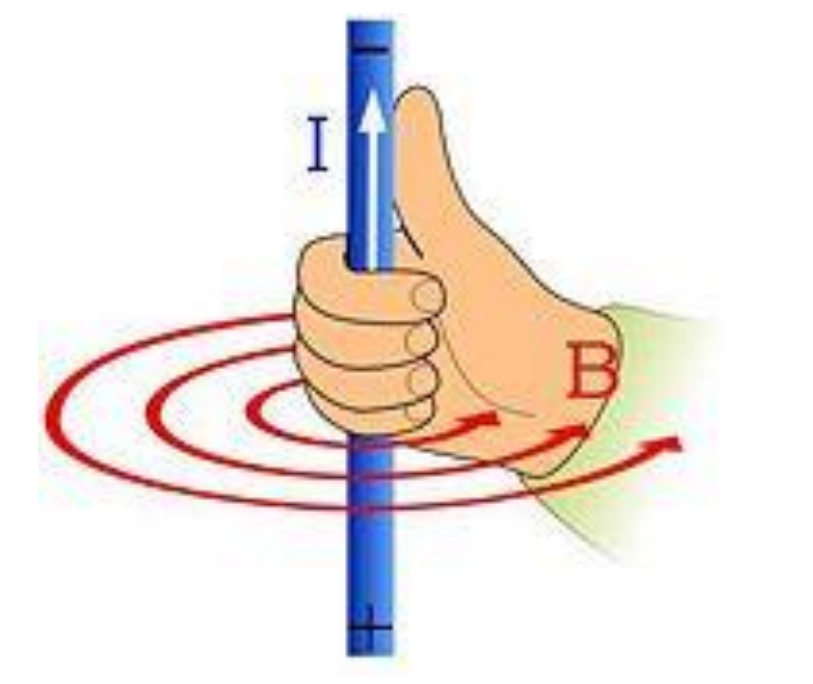
\includegraphics[scale=0.2]{img/rechte-hand-regel.png}}
	\end{center}
	\iend

	\definition{Lorentzkraft}
	\beginip
	Bewegte Ladungen in einem Magnetfeld verspüren eine Kraft, welche proportional zur Stärke des B-Feldes und der Geschwindigkeit ist. \\
	Die Kraft steht senkrecht zu den Feld- und Geschwindigkeits-Vektoren.

	\formulaBegin
	$\vec{F_L} = q \cdot \vec{v} \times \vec{B} = I(\vec{l} \times \vec{B})$
	\formulaEnd

	\begin{center}
			\ibox{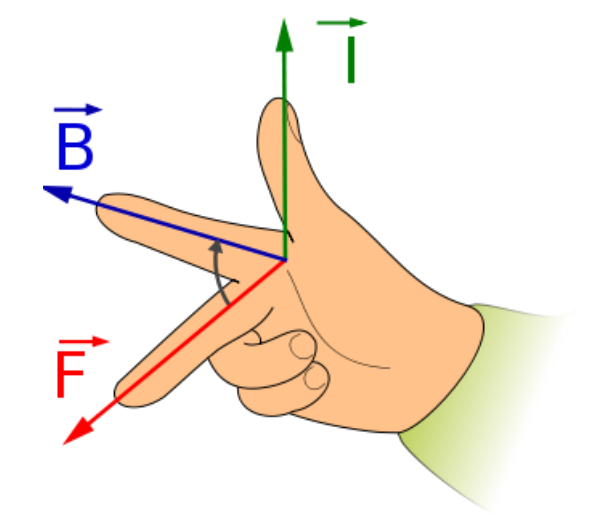
\includegraphics[scale=0.3]{img/lorentzkraft.png}}
	\end{center}
	\iend

\newpage
	\definition{H-Feld}
	\beginip
	Legen wir ein magnetisches Feld an eine Materie an, so richten sich die eingeschlossenen Teile entgegen dem angelegten Feld aus und \texttt{"} schwächen \texttt{"} dieses. \\
	Das \texttt{"} abgeschwächte \texttt{"} Feld bezeichnen wir als H-Feld und entspricht dem Feld, welches real auf Ladungen wirkt. \\
	 Der \texttt{"}Abschwächungsfaktor\texttt{"} $\mu = \mu_0 \cdot \mu_r$ wird als Permeabilität bezeichnet. \\
	 Das H-Feld verändert sich bei Materialübergängen, das \textbf{B-Feld} bleibt \textbf{konstant}.

	\formulaBegin
	$\displaystyle \vec{H} = \frac{\vec{B}}{\mu}$
	\formulaEnd

	\begin{center}
			\ibox{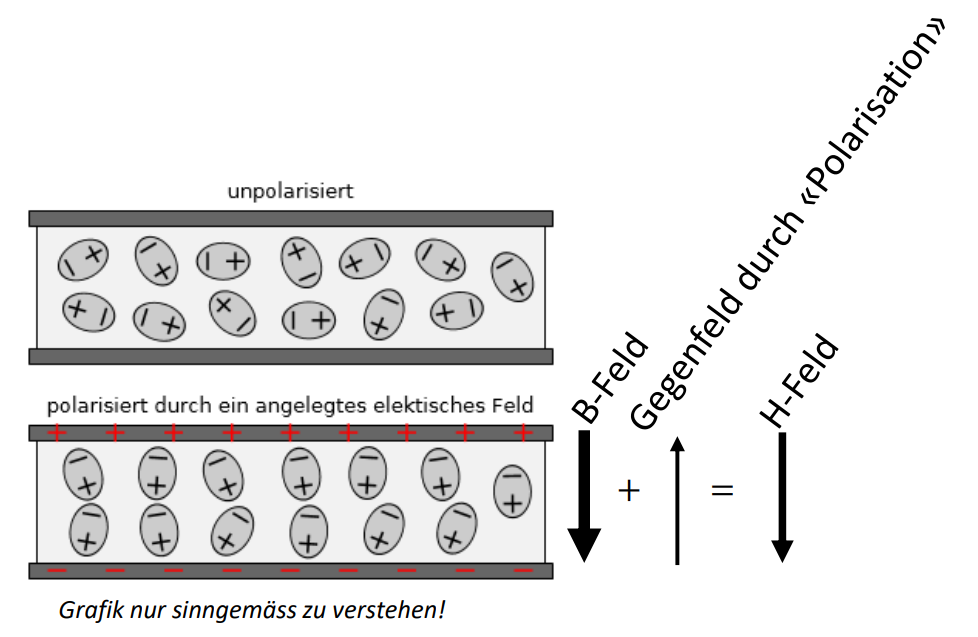
\includegraphics[scale=0.4]{img/h-feld.png}}
	\end{center}
	\iend

	\definition{Durchflutungssatz}
	\beginip
	Der Durchflutungssatz besagt, dass das Kurvenintegral des H-Feldes über eine beliebige \textbf{geschlossene} Kurve gerade dem Wert des durch diese Fläche fließendes Stromes entspricht. \\
	Diesen Wert definieren wir als magnetische Spannung $\Theta$ \\
	\formulaBegin
	$\displaystyle \Theta = \oint_{\partial A} \vec{H} \cdot d\vec{s} = \iint_{A} \vec{j} \cdot d\vec{A} $
	\formulaEnd
	\iend

	\important{Beispiel}{\#4}
	\beginip
	\textbf{Aufgabe} \\
	Berechnen Sie die magnetische Spannung $\Theta$ und das H-Feld Feld $\vec{H}$ um einen unendlich langen, mit Strom I durchflossenen Leiter. Der Radius des Leiters sei $\rho$. \\
	\iend

	\beginip
	\textbf{Lösung} \\

	Wir wählen als Kurve einen Kreis mit Radius R um unseren Leiter. \\
	Da wir von einem perfekten Leiter ausgehen, treffen wir die Annahme, dass das Magnetfeld achsensymmetrisch und somit konstant entlang des Kreises ist. \\
	\\
	Wir erhalten: für R $ > \rho$: \\
	$\displaystyle  \doubleunderline{\Theta} =  \oint_{2\pi R} \vec{H} \cdot d\vec{S} = \doubleunderline{I} $ \\
	$ \displaystyle \rightarrow |H| \cdot 2 \pi R = I \rightarrow \doubleunderline{\vec{H}(R) = \frac{I}{2 \pi R} \cdot \vec{e_{\varphi}}} $\\

	Für R $ < \rho $ : \\
	$\displaystyle  \doubleunderline{\Theta(R)} =  \oint_{2\pi R} \vec{H} \cdot d\vec{S} =\int_{0}^{R} \int_{0}^{2\pi} \frac{I}{\pi{\rho}^2} \cdot r \cdot d\varphi  \cdot dr  = \frac{2 \cdot I}{\rho^2} \cdot \frac{1}{2} R^2 =  \doubleunderline{\frac{R^2\cdot I}{\rho^2}} 		  $ \\
	$ \displaystyle \rightarrow |H| \cdot 2 \pi R = \frac{I \cdot R^2}{\rho^2} \rightarrow \doubleunderline{\vec{H}(R) = \frac{I}{2\pi \rho^2} \cdot R \cdot \vec{e_{\varphi}}} $

	\textbf{Skizze}
	\begin{center}
		\ibox{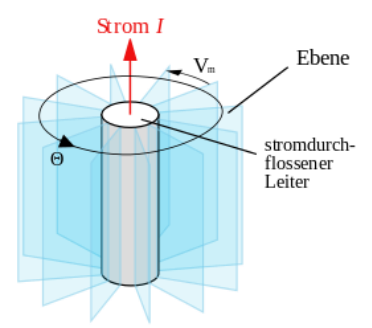
\includegraphics[scale=0.7]{img/ex4-1.png}}
	\end{center}
	\iend

	\important{Magnetische Spannung innerhalb einer Spule}{}

	\beginip
	Analog zu den Berechnungen beim Leiter kann man die magnetische Spannung innerhalb einer Spule berechnen. Unter der Annahme, dass das magnetische Feld ausserhalb des Spule vernachlässigbar ist
	und die Spule N Windungen hat, erhalten wir für den Fluss durch das Innere einer Spule:

	\formulaBegin
	$\displaystyle \Theta_{Spule} = \oint_{\partial A} \vec{H} \cdot d\vec{s} = \iint_{A} \vec{j} \cdot d\vec{A} = N \cdot I \simeq \int_0^b \vec{H} \cdot d\vec{s}$
	\formulaEnd
	\begin{center}
		\ibox{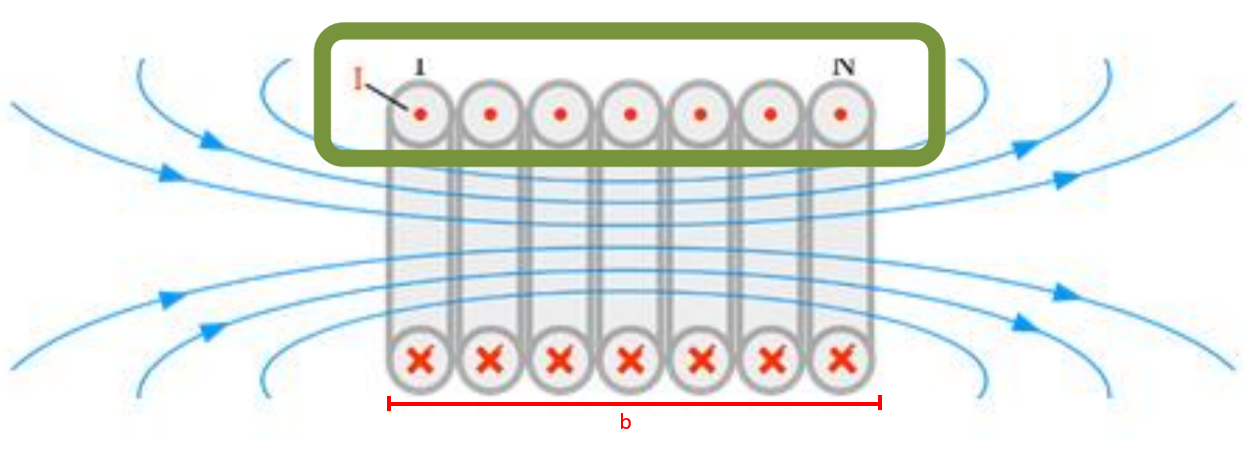
\includegraphics[scale=0.3]{img/spule_fluss.png}}
	\end{center}
	\iend

	Im folgenden gehen wir davon aus, dass die magnetische Spannung ungefähr $ \Theta = \int_0^l \vec{H} d\vec{s}$ entspricht.\\
	\definition{magnetischer Fluss}
	\beginip
		Als magnetischen Fluss $\Phi$ bezeichnen wir die \texttt{"}Menge B-Feld\texttt{"}, welche durch eine gegebene Fläche fliesst. \\
		\formulaBegin
		$\displaystyle \Phi := \iint_A \vec{B} \cdot \vec{n} \cdot da$
		\formulaEnd
	\iend


	\definition{magnetischer Widerstand}
		\beginip
			Als magnetischer Widerstand $R_m$ bezeichnen wir das Verhältnis zwischen magnetischer Spannung und magnetischem Fluss \\
			Er sagt etwas darüber aus, wie gross der magnetische Fluss bei einer gegebenen magnetischen Spannung ist.
			\formulaBegin
			$\displaystyle R_m = \frac{\Theta}{\Phi} \underbrace{=}_{magn. Leiter} \frac{l}{\mu \cdot A}$
			\formulaEnd
		\iend

		\textbf{Begründung} \\
		Wir gehen davon aus, dass die magnetische Spannung über einem Leiter mit Länge l anliegt, dessen Querschnittfläche A ist. \\
		\begin{center}
			$\displaystyle \frac{\Theta}{\Phi} = \frac{\int_0^l \vec{H} \cdot d\vec{s}}{\iint_a \vec{B} d \vec{A}} = \frac{l \cdot H}{\mu \cdot A \cdot H} = \frac{l}{\mu \cdot A} $

		\end{center}


\newpage

\subsubsection{Das Reluktanzmodell}
		\textbf{magnetische Grössen im Vergleich zu eletrischen} \\

		\def\arraystretch{2}%  1 is the default, change whatever you need
		\begin{tabular}{c|c|c||c|c}
			& Elektrisch & Einheit & Magnetisch & Einheit \\
			\hline
			\hline
			Leitfähigkeit & $ \kappa $ & $\texttt{[}   \frac{1}{\Omega \cdot m}    \texttt{]}$ & $\mu (= \mu_0 \cdot \mu_r)$ & $\texttt{[}  \frac{H}{m}\texttt{]}$ \\
			Widerstand & $ R = \frac{l}{\kappa A} $ & $\texttt{[}   \Omega   \texttt{]}$ & $R_m = \frac{l}{\mu A}$ & $\texttt{[} \frac{1}{H}\texttt{]}$ \\
			Leitwert & $ G = \frac{1}{R} $ & $\texttt{[}  S \texttt{]}$ & $\Lambda_m = \frac{1}{R_m}$ & $\texttt{[}  H  \texttt{]}$ \\
			\hline


			Spannung & $\displaystyle U_{AB} = \int_A^B \vec{E} \cdot d\vec{s}$ & $\texttt{[}V\texttt{]}$ & $\displaystyle \Theta_{AB}= \int_A^B \vec{H} \cdot d\vec{s}$ &  $\texttt{[}A\texttt{]}$ \\
			Strom / Fluss & $\displaystyle I = \iint_A \vec{j}\cdot d\vec{A} = \kappa \iint_A \vec{E} \cdot d\vec{A}$ & $\texttt{[}A\texttt{]}$  & $ \iint_A \vec{B} \cdot d \vec{A} = \mu \iint_A \vec{H} \cdot d\vec{A}$ &  $\texttt{[}Wb\texttt{]}$ \\
			\hline
			Ohmsches Gesetz & $U = R \cdot I $ &  & $\Theta = R_m \cdot \Phi $ &  \\
			Maschenregel & $ U_0 = \sum_{Masche} U_m $ &  & $ \Theta(= NI) = \sum_{Masche} \Theta_m $ & \\
			Knotenregel & $ \sum_{Knoten} I_k = 0 $ &  & $ \sum_{Knoten} \Phi_k = 0 $ &  \\

		\end{tabular}

		\definition{Reluktanzmodell}
		\beginip
		Das Reluktanzmodell besagt, dass man ein magnetisches Ersatzschaltbild mit denselben Rechenregeln wie bei einem elektrischen Netzwerk berechnen kann. \\
		\textbf{Vorgehen} \\
		\begin{itemize}
			\item Spulen werden mit Spannungsquellen ersetzt $V_m = N\cdot I$
			\item Magnetkerne/Luftspälte etc. werden mithilfe der Länge und Querschnittsfläche als Widerstände modelliert. $R_m = \mu \frac{l}{A}$
			\item Für magnetische Widerstände gelten die gleichen Regeln wie bei elektrischen (Seriellschaltung / Paralellschaltung).
		\end{itemize}

		\iend
\newpage
		\important{Beispiel}{\#5}
		\beginip
 		\textbf{Aufgabe Hubmagnet} \\
		Der mittlere Schenkel 2 eines E-Kernes aus Dynamoblech trägt eine Wicklung mit N Windungen. Über
		die drei Luftspalten mit gleicher Länge $\delta$ wird ein Anker aus Grauguss mit der Kraft FA angezogen
		E-Kern und Anker besitzen die gleiche Dicke d. \\
		\begin{center}
		\ibox{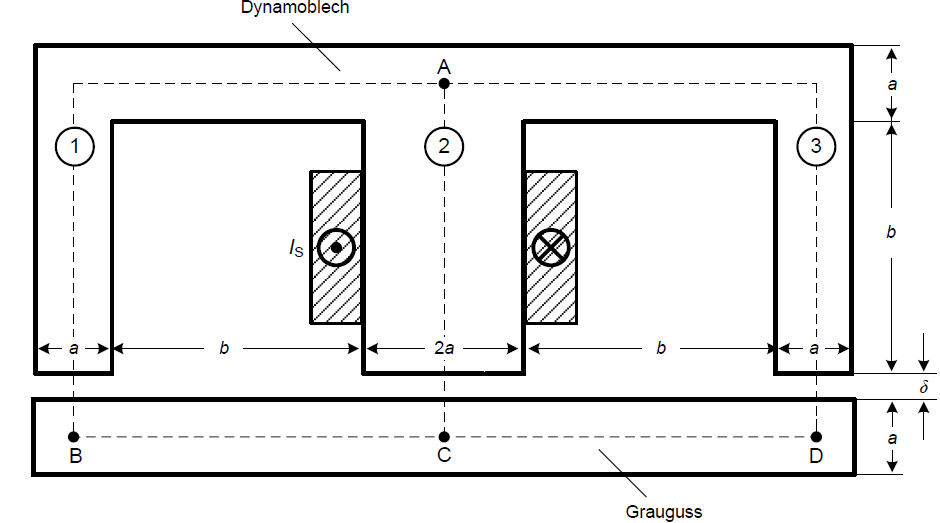
\includegraphics[scale=0.4]{img/ex5-1.png}}
		\end{center}
		Gegeben sind folgende Parameter: \\

		\begin{center}
	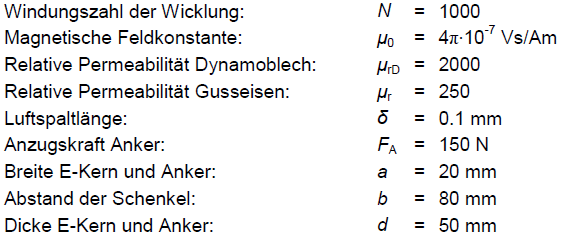
\includegraphics[scale=0.6]{img/ex5-3.png}
		\end{center}
		Berechnen sie die magnetische Spannung auf dem Weg ACD.
		\iend

\newpage
		\important{Lösung}{}
				\beginip
		Zuerst zeichnen wir ein Reluktanzmodell des Magneten. \\
		Wobei $R_L$ die Luftspälte, ${R_D}_i$ die Beine des Magneten und ${R_G}_i$ sowie $R_{BC}$ und $R_{CD}$ das Gusseinsenstück modellieren.
	\begin{center}
			\ibox{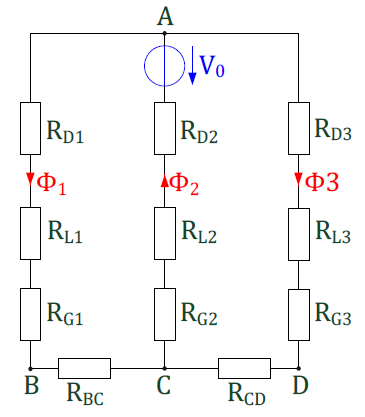
\includegraphics[scale=0.5]{img/ex5-2.png}}
			\end{center}


		Für die Spannungsquelle erhalten wir:
			\begin{center}

				 $V_0 = N \cdot I_s = 1000 \cdot 211.3mA = 211.3A$ \\
			\end{center}
		Für die Widerstände:
			\begin{center}
	 	$R_{D1} = R_{D3} = \frac{2b + 2a}{\mu_0 \mu_{rD} a d} = 79.6 \cdot 10^3H^{-1}$ \\
	 	$R_{D2} = \frac{b + \frac{a}{2} }{2 \mu_0 \mu_{rD} a d} = 17.9 \cdot 10^3H^{-1}$ \\

	 	$R_{L1} = R_{L3} = \frac{\delta}{\mu_0 a d} = 79.6 \cdot 10^3H^{-1}$ \\
		$R_{L2} =  \frac{\delta}{2\mu_0 a d} = 39.8 \cdot 10^3 H^{-1}$\\
		$R_{G1} = R_{G3} = \frac{\frac{a}{2}}{\mu_0\mu_{rG}ad} = 31.8 \cdot 10^3H^{-1}$ \\
		$R_{G2} =\frac{\frac{a}{2}}{2\mu_0\mu_{rG}ad} = 15.9 \cdot 10^3H^{-1}$ \\
		$R_{BC} = R_{CD} = \frac{b + \frac{3}{2}a}{2\mu_0\mu_{rG}ad} = 350.1\cdot 10^3H^{-1}$ \\
				\end{center}
		Weiter können wir die einzelnen Widerstände seriell zusammenfassen:
			\begin{center}
		$R_1 = R_{D1} + R_{L1} + R_{G1} = 191 \cdot 10^3 H^{-1}$ \\
		$R_2 = R_{D2} + R_{L2} + R_{G2} = 73.7 \cdot 10^3 H^{-1}$ \\
		$R_3 = R_{D3} + R_{L3} + R_{G3} = 191 \cdot 10^3 H^{-1}$ \\
		$R_E = R_{BC} = R_ {CD} = 350.1 \cdot 10^3 H^{-1} $ \\
					\end{center}

		Die Spannung $U_{AC}$ lässt sich als Spannungsteiler berechnen:

			\begin{center}
		$\displaystyle U_{AC} = U_0 \cdot \frac{((R_1 + R_E) || (R_3 + R_E)) } { ((R_1 + R_E) || (R_3 + R_E)) + R_2} = 166A$ \\
				\end{center}
		Und somit die Spannung $ U_{AD}$:
		\begin{center}
			$\displaystyle \doubleunderline{U_{AD}} = 166A \cdot \frac{R_1}{R_1 + R_E} = \doubleunderline{58.6A}$
		\end{center}
		\iend

\newpage

\subsection{Spule und Induktivität}

\definition{Induktivität}
\beginip
	Die Induktivität L beschreibt, wieviel magnetischer Fluss $\Phi$ sich bei einem Strom I im Inneren eines Bauteiles aufbaut.
	\formulaBegin
	$ L := \frac{N\cdot \Phi}{I} = \frac{N^2}{R_m} $
	\formulaEnd
	Die in einer Induktivität gespeicherte Energie berechnet sich zu
	\formulaBegin
	$W =\displaystyle \frac{1}{2}L \cdot I^2$
	\formulaEnd
\iend



	\definition{Serien und Parallelschaltung}
	 \beginip
	 	Induktivitäten verhalten sich analog zu Widerständen: \\
		\textbf{Serienschaltung}
		\formulaBegin
		$ L_{serie} = \sum_{i=0}^n L_i $
		\formulaEnd

		\textbf{Parallelschaltung}
		\formulaBegin
		$\displaystyle \frac{1}{L_{ges}} = \sum_{i=0}^n \frac{1}{L_i} \Bigg\rvert L_{p_2} = (L_1 || L_2 )$
		\formulaEnd
	 \iend


	\textbf{Übersicht} \\
	\\
	\begin{tabular}{|c|c|c|c|c|}
	\hline
		\textbf{Energie} & 	\textbf{Strom und Spannung} & 	\textbf{ DC-Verhalten} & 	\textbf{ High-AC Verhalten*}& 	\textbf{ Admitanz*} \\
		\hline 	\hline
		 & & & & \\
	    $ \displaystyle L =  \frac{N \Phi}{I} $ & $\displaystyle i_L(t) = \frac{1}{L} \int_0^t u_c(t) dt $ & Leerlauf & Kurzschluss & $ \displaystyle j\omega L$  \\
		  $\displaystyle W =  \frac{1}{2} L I^2 $ & $\displaystyle u_L(t) = L \cdot \frac{d}{d t} (i_c) $ & 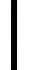
\includegraphics[scale=0.5]{img/kurzschluss} &   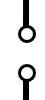
\includegraphics[scale=0.4]{img/leerlauf}  &   \\
			 & & & & \\
			\hline
	\end{tabular}
